% Walmart Medallion Data Pipeline — Comprehensive Technical Report
% Engine: pdfLaTeX / XeLaTeX / LuaLaTeX (all compatible)
% Compile: pdflatex report.tex && pdflatex report.tex   (or latexmk -pdf)
\documentclass[11pt,a4paper]{article}

% ------------------------------------------------------------------ layout
\usepackage[a4paper,margin=2.2cm,top=2.3cm,bottom=2.3cm]{geometry}
\usepackage[utf8]{inputenc}
\usepackage[T1]{fontenc}
\usepackage{lmodern}
\usepackage{enumitem}
\usepackage{booktabs}
\usepackage{longtable}
\usepackage{array}
\usepackage{graphicx}
\usepackage{xcolor}
\usepackage{listings}
\usepackage{hyperref}
\usepackage{amsmath,amssymb}
\usepackage{tikz}
\usepackage{fancyhdr}
\usepackage{titlesec}
\usepackage{float}
\usepackage{caption}
\usepackage{parskip}
\usetikzlibrary{shapes.geometric,arrows.meta,positioning,calc,shadows}

% ------------------------------------------------------------------ colours
\definecolor{walmartBlue}{HTML}{0071CE}
\definecolor{walmartYellow}{HTML}{FFC220}
\definecolor{bronzeC}{HTML}{8B5A2B}
\definecolor{silverC}{HTML}{6B7280}
\definecolor{goldC}{HTML}{92400E}
\definecolor{ink}{HTML}{0F172A}
\definecolor{muted}{HTML}{64748B}
\definecolor{line}{HTML}{E2E8F0}
\definecolor{codeBg}{HTML}{F8FAFC}

% ------------------------------------------------------------------ hyperref
\hypersetup{
  colorlinks=true,
  linkcolor=walmartBlue,
  urlcolor=walmartBlue,
  citecolor=walmartBlue,
  pdftitle={Walmart Medallion Pipeline — Technical Report},
  pdfauthor={Nitin},
  pdfsubject={MongoDB → PostgreSQL medallion ETL, dbt, Airflow, Docker}
}

% ------------------------------------------------------------------ header / footer
\pagestyle{fancy}
\fancyhf{}
\fancyhead[L]{\small\textsc{Walmart Medallion Pipeline}}
\fancyhead[R]{\small Technical Report — 2026}
\fancyfoot[C]{\small\thepage}
\renewcommand{\headrulewidth}{0.4pt}
\renewcommand{\footrulewidth}{0pt}

% ------------------------------------------------------------------ section style
\titleformat{\section}{\Large\bfseries\color{ink}}{}{0em}{}[\vspace{0.2em}\hrule height 0.6pt \vspace{0.4em}]
\titleformat{\subsection}{\large\bfseries\color{ink}}{}{0em}{}
\titleformat{\subsubsection}{\normalsize\bfseries\color{ink}}{}{0em}{}
\titlespacing*{\section}{0pt}{1.2em}{0.6em}
\titlespacing*{\subsection}{0pt}{0.9em}{0.4em}

% ------------------------------------------------------------------ listings
\lstdefinestyle{sql}{
  language=SQL,
  backgroundcolor=\color{codeBg},
  basicstyle=\ttfamily\small,
  keywordstyle=\color{walmartBlue}\bfseries,
  commentstyle=\color{muted}\itshape,
  stringstyle=\color{goldC},
  showstringspaces=false,
  breaklines=true,
  frame=single,
  rulecolor=\color{line},
  tabsize=2,
  captionpos=b,
  numbers=none,
}
\lstdefinestyle{py}{
  language=Python,
  backgroundcolor=\color{codeBg},
  basicstyle=\ttfamily\small,
  keywordstyle=\color{walmartBlue}\bfseries,
  commentstyle=\color{muted}\itshape,
  stringstyle=\color{goldC},
  showstringspaces=false,
  breaklines=true,
  frame=single,
  rulecolor=\color{line},
}
\lstdefinestyle{bash}{
  language=bash,
  backgroundcolor=\color{codeBg},
  basicstyle=\ttfamily\small,
  keywordstyle=\color{ink},
  commentstyle=\color{muted}\itshape,
  showstringspaces=false,
  breaklines=true,
  frame=single,
  rulecolor=\color{line},
}

% ------------------------------------------------------------------ title
\title{
  \vspace{1.2cm}
  {\Huge\bfseries Walmart Medallion Data Pipeline\par}
  \vspace{0.35cm}
  {\Large MongoDB $\rightarrow$ PostgreSQL $\rightarrow$ dbt \quad (Bronze $\rightarrow$ Silver $\rightarrow$ Gold)\par}
  \vspace{0.45cm}
  {\large Incremental PySpark Extraction \,|\, 17 dbt Models \,|\, 3 Runners \,|\, 8 Quality Gates\par}
}
\author{
  Nitin \quad\textcolor{muted}{— Walmart\_DBT}
}
\date{
  September 2026 \quad\textcolor{muted}{\textbar\quad} v0.1.0 \quad\textcolor{muted}{\textbar\quad}
  \href{https://github.com/Nitinx12/Walmart_DBT}{github.com/Nitinx12/Walmart\_DBT}
}

% ================================================================ DOCUMENT
\begin{document}
\maketitle
\thispagestyle{empty}
\begin{center}
  
\begin{tikzpicture}[node distance=1.2cm]
    \node[draw=walmartBlue,fill=walmartBlue!7,rounded corners=8pt,inner sep=8pt,minimum width=13cm,align=center] (box) {
      \small\textcolor{muted}{One pipeline, three runners — } \textbf{PowerShell}, \textbf{Airflow DAG}, \textbf{Docker image}
      \quad\textcolor{muted}{\textbar}\quad
      \textcolor{muted}{One warehouse — } \textbf{walmart\_db} \textcolor{muted}{with schemas} \textbf{bronze / silver / gold}
    };
  \end{tikzpicture}
\end{center}
\vspace{0.6cm}
\begin{abstract}
\noindent
This report documents the production-style medallion ETL that mirrors MongoDB operational data into a PostgreSQL warehouse and curates it through \texttt{bronze} (raw, 1:1), \texttt{silver} (deduped, typed, SCD2) and \texttt{gold} (dimensional star/snowflake) layers. The pipeline is implemented once and executed identically by three runners — \texttt{pipeline/run\_pipeline.ps1} (Windows host), a standalone Docker image (\texttt{main.py}), and an Airflow DAG (\texttt{airflow/dags/walmart\_pipeline\_dag.py}) — over eight strict stages gated by two independent test systems plus Great Expectations. It covers 9 silver and 8 gold dbt models, watermark-based incremental extraction with true upserts, containerisation with two images, CI with a live Postgres integration job, and a Streamlit+Plotly gold dashboard. All commands use \texttt{uv} and \texttt{uv.lock} is the source of truth.
\end{abstract}
\vspace{0.3cm}
\begin{center}
\small\textcolor{muted}{Keywords —} Medallion architecture, PySpark, MongoDB Spark Connector, PostgreSQL 16, dbt Core, Airflow 3.3, Great Expectations, Docker Compose, Streamlit
\end{center}
\newpage
\tableofcontents
\newpage

% ================================================================= 1
\section{Introduction \& Objectives}

\subsection{Why medallion}
Operational MongoDB must stay write-optimised; analytics needs a typed, historical, dimensional warehouse. The medallion pattern isolates those concerns: \textbf{bronze} preserves source fidelity, \textbf{silver} enforces types and slowly-changing history, \textbf{gold} publishes a star schema for BI. Every hand-off between layers is a quality gate — downstream layers only build if the upstream gate passes.

\subsection{Project goals}
\begin{enumerate}[leftmargin=1.4em,itemsep=2pt]
  \item Replicate \emph{every} user collection from MongoDB to Postgres automatically (no hard-coded list) and keep it incrementally fresh without re-copying unchanged data.
  \item Cure source issues once (typing, deduplication, SCD2) so gold consumers never re-implement cleaning.
  \item Publish a dimensional star (\texttt{fact\_order\_items} + 7 dims) that powers both SQL reports (\texttt{sql/*.sql}) and an interactive dashboard.
  \item Gate quality twice at each hand-off: dbt built-ins (\texttt{schema.yml}) \emph{and} a standalone SQL suite (\texttt{tests/bronze|silver|gold}), plus a final cross-layer Great Expectations checkpoint.
  \item Run the \emph{same} logic three ways — local Windows, Airflow schedule, standalone container — without forking code.
  \item Ship like a team would: \texttt{uv} lockfile, Ruff + SQLFluff + pre-commit, GitHub Actions CI with a live Postgres integration job, Docker images published to GHCR.
\end{enumerate}

\subsection{Non-goals}
Real-time streaming (this is batch incremental), cross-warehouse federation, and PII masking are out of scope for the current milestone.

% ================================================================= 2
\section{Architecture at a Glance}

\begin{center}
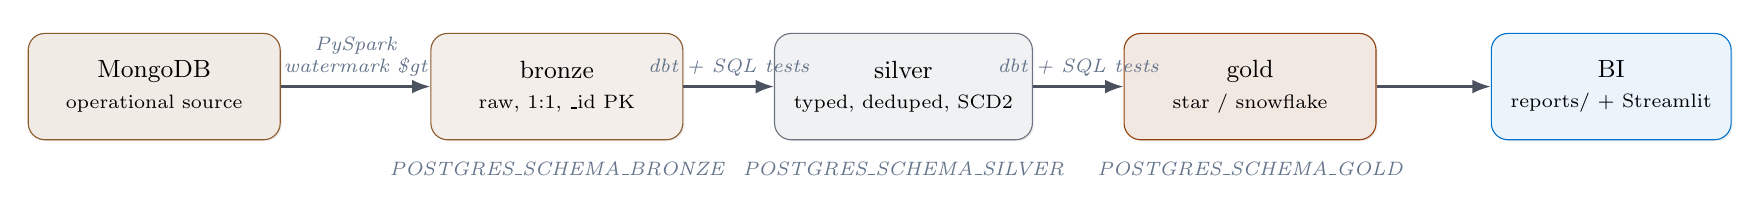
\begin{tikzpicture}[
  box/.style={draw,rounded corners=6pt,inner sep=7pt,minimum width=3.2cm,minimum height=1.35cm,align=center,font=\small,drop shadow={shadow xshift=0.6pt,shadow yshift=-0.6pt,opacity=0.12}},
  arr/.style={-Latex,thick,color=ink!75},
  lbl/.style={font=\scriptsize\itshape,color=muted,align=center}
]
  \node[box,fill=bronzeC!12,draw=bronzeC] (mongo) {MongoDB\\{\scriptsize operational source}};
  \node[box,fill=bronzeC!10,draw=bronzeC,right=1.9cm of mongo] (bronze) {bronze\\{\scriptsize raw, 1:1, \_id PK}};
  \node[box,fill=silverC!10,draw=silverC,right=1.15cm of bronze] (silver) {silver\\{\scriptsize typed, deduped, SCD2}};
  \node[box,fill=goldC!12,draw=goldC,right=1.15cm of silver] (gold) {gold\\{\scriptsize star / snowflake}};
  \node[box,fill=walmartBlue!8,draw=walmartBlue,right=1.45cm of gold,minimum width=3.0cm] (bi) {BI\\{\scriptsize reports/ + Streamlit}};
  \draw[arr] (mongo) -- node[lbl,above]{PySpark \\ watermark \$gt} (bronze);
  \draw[arr] (bronze) -- node[lbl,above]{dbt + SQL tests} (silver);
  \draw[arr] (silver) -- node[lbl,above]{dbt + SQL tests} (gold);
  \draw[arr] (gold) -- (bi);
  \node[lbl,below=0.15cm of bronze] {POSTGRES\_SCHEMA\_BRONZE};
  \node[lbl,below=0.15cm of silver] {POSTGRES\_SCHEMA\_SILVER};
  \node[lbl,below=0.15cm of gold] {POSTGRES\_SCHEMA\_GOLD};
\end{tikzpicture}
\end{center}

Postgres database is \texttt{walmart\_db}. Medallion schemas default to \texttt{bronze / silver / gold} via \texttt{POSTGRES\_SCHEMA\_*} in \texttt{.env} (\texttt{.env.example:1} is the template). Control tables \texttt{etl\_watermarks} and \texttt{etl\_logs} live alongside bronze collections. All runners set \texttt{PYTHONPATH} to the project root so \texttt{utils.*} resolves identically.

% ================================================================= 3
\section{Technology Stack}

\begin{longtable}{>{\bfseries}l l l}
\toprule
Layer & Technology & Version / Notes \\
\midrule
\endhead
Language & Python & 3.13 local, 3.12-slim Docker, 3.11 CI \\
Package mgr & uv & \texttt{uv.lock} is source of truth; never hand-edit \texttt{pyproject.toml} without \texttt{uv lock} \\
Compute & PySpark & 3.5.5 (pinned) — required by \texttt{mongo-spark-connector\_2.12:10.4.0}; 4.x is binary-incompatible (SPARK-4 Catalyst change) \\
Source & MongoDB & Operational DB, auto-discovered collections \\
Warehouse & PostgreSQL & 16 — \texttt{walmart\_db}, JDBC via \texttt{jars/postgresql.jar} \\
Transform & dbt Core + dbt-postgres & 1.12.0 / 1.11.0 — 17 models, 100+ tests \\
Orchestration & Apache Airflow & 3.3.x, CeleryExecutor (scheduler, worker, triggerer, Redis, Postgres meta DB) \\
Quality & Great Expectations & 1.21.0 — suites per layer in \texttt{pipeline/data\_quality/suites/} \\
BI & Streamlit 1.62 + Plotly 7.0 & Live gold dashboard at \texttt{dashboard/app.py} \\
Lint / Format & Ruff 0.16 + SQLFluff 4.2 + pre-commit & \texttt{ruff check / format}, \texttt{sqlfluff lint --dialect postgres} \\
Containers & Docker / Compose & \texttt{docker/Dockerfile} (standalone) + \texttt{docker/Dockerfile.airflow} \\
CI & GitHub Actions & lint $\rightarrow$ dashboard-smoke $\rightarrow$ unit $\rightarrow$ DAG $\rightarrow$ Docker $\rightarrow$ integration (live Postgres) \\
\bottomrule
\end{longtable}

JDK is 17 (\texttt{docker/Dockerfile} and dev container) — PySpark 3.5's Mongo connector is untested on JDK 21, so the pin is intentional (\texttt{AGENTS.md} convention).

% ================================================================= 4
\section{Repository Layout}

\begin{lstlisting}[style=bash,caption={Top-level layout (trimmed). Mirrors \texttt{docs/architecture.md}.}]
airflow/        dags/walmart_pipeline_dag.py + logs/plugins/config (bind-mounted)
docker/         Dockerfile, Dockerfile.airflow, compose.yml, dbt/profiles.yml, entrypoint.sh
docs/           architecture.md, airflow.md, dbt.md, docker.md, pipeline.md, scripts.md, ...
jars/           mongo-spark-connector + deps (5 jars) + postgresql.jar (offline Spark startup)
pipeline/       run_pipeline.ps1  (+ .bat shim), data_quality/{run.py, context.py, suites/}
scripts/python/ extract.py, sql_test.py, ci_seed_bronze.py, health_check.py, seed_demo_db.py, ...
scripts/bash/   preflight.sh, run_pipeline.sh, run_tests.sh, health.sh, security.sh, ...
sql/            00_init_schema.sql .. 20_no_sales_date_analysis.sql (hand-written reports)
tests/          bronze/ (3), silver/ (9), gold/ (7)  — standalone SQL suite
utils/          engine.py (env validation), connection.py (cached), logger.py
dbt/            dbt_project.yml, models/{silver,gold}, seeds, snapshots, macros
dashboard/      app.py, queries.py, components.py, theme.py
reports/        brand_report.md, category_report.md, report.tex (this file) -> report.pdf
main.py         standalone Docker entry point (mirrors ps1 stage-for-stage)
\end{lstlisting}

Coding conventions: \texttt{snake\_case}, type hints on every signature, one function = one responsibility (see \texttt{scripts/python/extract.py} stage split), short \texttt{// why not what} comments, \texttt{uv run ruff format/check} before commit.

% ================================================================= 5
\section{Pipeline — Eight Strict Stages}

The pipeline has a fixed order. If stage order or the definition of ``success'' changes, \texttt{pipeline/run\_pipeline.ps1} \emph{and} \texttt{airflow/dags/walmart\_pipeline\_dag.py} must change together (convention, not enforced — \texttt{AGENTS.md: Pipeline Stage Rule}).

\begin{center}
\begin{longtable}{cl l l}
\toprule
\# & Stage & Runner command & Gate \\
\midrule
\endhead
0 & Preflight & \texttt{uv run python -c "import pyspark; print(...)"} + prefix check \texttt{3.5.x} & Version mismatch $\rightarrow$ fail fast (ps1) / install guard (container refuses to self-heal) \\
1 & Extract & \texttt{uv run python scripts/python/extract.py} & Per-collection \texttt{VALIDATION FAILED} $\rightarrow$ non-zero exit \\
2 & Bronze SQL tests & \texttt{uv run python scripts/python/sql\_test.py tests/bronze} & 3 checks; any violating rows $\rightarrow$ FAIL \\
3 & dbt silver & \texttt{cd dbt \&\& uv run dbt run --select silver} \newline \texttt{uv run dbt test --select silver} & \texttt{schema.yml} tests; \texttt{dbt test} failure stops stage \\
4 & Silver SQL tests & \texttt{.../sql\_test.py tests/silver} & 9 checks \\
5 & dbt gold & \texttt{uv run dbt run --select gold} + \texttt{test} & 8 models, 7 dims + 1 fact \\
6 & Gold SQL tests & \texttt{.../sql\_test.py tests/gold} & 7 checks \\
7 & Great Expectations & \texttt{uv run python -m pipeline.data\_quality.run --layer all} & Bronz/Silver/Gold suites; exit 1 = data failure, 2 = build error \\
\bottomrule
\end{longtable}
\end{center}

\textbf{Stop-on-first-failure:} \texttt{run\_pipeline.ps1:99} (\texttt{Stop-Pipeline}) and \texttt{main.py:244} (\texttt{raise}) halt immediately; Airflow's default \texttt{all\_success} trigger does the same — downstream tasks go to \texttt{upstream\_failed} with no extra guard.

PowerShell, Python, and Airflow share one mental model: the header ``\texttt{STEP n / 7}'' (\texttt{main.py:37 TOTAL\_STEPS = 7} plus stage 0 = 8 stages) stays honest via an assert. Logs go to \texttt{logs/pipeline\_YYYY-MM-DD.log} (\texttt{utils/logger.py}) plus \texttt{\{schema\}.etl\_logs} audit rows.

% ================================================================= 6
\section{Bronze Ingestion — Watermark Extraction in Detail}

\texttt{scripts/python/extract.py} ($\approx$1230 lines) is the only place that touches MongoDB.

\subsection{Auto-discovery}
\texttt{discover\_collections()} lists \texttt{mongo\_db.list\_collection\_names()} and drops any name starting with \texttt{system.} (\texttt{extract.py:127}). No collection list is ever hard-coded, and \texttt{--tables} is an optional filter for ad-hoc runs.

\subsection{Watermark column priority}
Per collection, a single document sample is inspected and the first present candidate wins:
\begin{center}
\texttt{updated\_timestamp} $\succ$ \texttt{updated\_at} $\succ$ \texttt{created\_timestamp} $\succ$ \texttt{created\_at} \quad (\texttt{extract.py:151})
\end{center}
\texttt{updated\_*} is preferred because documents mutated after insert (e.g. order status $\rightarrow$ \texttt{Cancelled}) must be re-synced, not just newly-inserted rows. If none is present, the collection falls back to full reload every run with a warning.

\subsection{Incremental pushdown}
When a watermark column and a prior \texttt{last\_watermark\_value} exist, the Spark read is filtered server-side:
\begin{lstlisting}[style=py,caption={Pushdown filter — string comparison is intentional}]
watermark_str = since.strftime("%Y-%m-%d %H:%M:%S")
pipeline = json.dumps([{"$match": {col: {"$gt": watermark_str}}}])
reader.option("aggregation.pipeline", pipeline)  # extract.py:656
\end{lstlisting}
The comparison is string-to-string because the source stores these timestamps as \texttt{"YYYY-MM-DD HH:MM:SS"} strings, not BSON dates — MongoDB never matches across BSON types in \texttt{\$gt}.

\subsection{Upsert, not append}
\texttt{\_id} (cast to string, \texttt{sanitize\_for\_postgres:672}) is the merge key. Existing tables get a scratch staging table \texttt{\_stg\_\{collection\}} written with \texttt{mode("overwrite")}, then a single
\begin{lstlisting}[style=sql,caption={Merge — inserted vs updated via xmin}]
WITH upsert AS (
  INSERT INTO "bronze"."orders" ("_id", ...) 
  SELECT ... FROM "bronze"."_stg_orders"
  ON CONFLICT ("_id") DO UPDATE SET ... 
  RETURNING (xmax = 0) AS inserted
)
SELECT count(*) FILTER (WHERE inserted) AS rows_inserted,
       count(*) FILTER (WHERE NOT inserted) AS rows_updated
FROM upsert;  -- extract.py:721
\end{lstlisting}
A unique index on \texttt{\_id} is ensured first (\texttt{ensure\_unique\_id\_index:409}); if creation fails (duplicate \_id from a prior append-only run), the run falls back to plain \texttt{append} and warns — never silently corrupts.

\subsection{Nested fields}
\texttt{StructType / ArrayType / MapType} columns are serialised to JSON strings via \texttt{to\_json()} (\texttt{extract.py:680}) — the only ``lossy'' step, required because plain JDBC has no native struct type. Flattened field names are reported in the Rich final panel.

\subsection{Control tables}
Both live in the bronze schema:
\begin{itemize}[leftmargin=1.4em]
  \item \texttt{\{bronze\}.etl\_watermarks} — one row per collection: \texttt{incremental\_column, last\_watermark\_value, last\_run\_mode, rows\_inserted/updated, updated\_at}. Upserted via \texttt{ON CONFLICT (table\_name)} (\texttt{extract.py:528}).
  \item \texttt{\{bronze\}.etl\_logs} — one audit row per collection per run: mode, counts before/after, validation status, \texttt{error\_full} traceback, duration. Best-effort, never fails the run.
\end{itemize}
\texttt{ensure\_control\_tables:448} is idempotent and forward-migrates columns added in later versions.

\subsection{Validation \& reporting}
After each merge, \texttt{validate\_collection:619} recounts the target and expects \texttt{before + inserted}. A Rich report prints per-collection rows, watermark state, flattened fields, and failures (\texttt{render\_report:916}); the same data lands in both the daily log file and \texttt{etl\_logs}.

CLI: \texttt{--tables}, \texttt{--full-refresh} (truncates before load), \texttt{--dry-run}, \texttt{--watermark-column} override (\texttt{extract.py:1117}).

% ================================================================= 7
\section{Silver Layer — Clean, Typed, Historical}

\texttt{dbt/dbt\_project.yml:35} materialises all silver models as \texttt{table} in schema \texttt{silver}. Nine models mirror bronze tables 1:1 but add:

\begin{center}
\begin{longtable}{l l l}
\toprule
Model & Key cleaning & Notable logic \\
\midrule
\endhead
\texttt{silver.brands} & dedup on \texttt{\_id}, trim/case normalisation & Coalesce brand name variants \\
\texttt{silver.categories} & dedup, null handling & Canonical category list \\
\texttt{silver.customers} & dedup, email lower, phone normalise & \texttt{is\_active} flag \\
\texttt{silver.employees} & dedup, date parsing & Joins to stores \\
\texttt{silver.orders} & timestamp parsing, status canonicalisation & \texttt{order\_timestamp} typed \\
\texttt{silver.order\_items} & \texttt{line\_amount = qty * unit\_price} recomputed & FK to orders + products \\
\texttt{silver.payment\_methods} & dedup, type normalisation & Lookup for gold dim \\
\texttt{silver.products} & dedup, price typing, FK checks & Links brands + categories \\
\texttt{silver.stores} & dedup, geo normalisation & Store master \\
\bottomrule
\end{longtable}
\end{center}

Each model has a \texttt{schema.yml} with \texttt{not\_null}, \texttt{unique}, \texttt{relationships} and \texttt{accepted\_values} tests. The silver grain is ``one row per source document'' — no aggregation yet.

\texttt{tests/silver/} contributes 9 additional PL/pgSQL checks (row counts, orphan FKs, distinctness) executed by \texttt{scripts/python/sql\_test.py}.

% ================================================================= 8
\section{Gold Layer — Dimensional Star / Snowflake}

\texttt{dbt/dbt\_project.yml:39} materialises gold as \texttt{table} in schema \texttt{gold}. Eight models:

\begin{center}
\begin{longtable}{l l p{7.2cm}}
\toprule
Model & Type & Grain \\
\midrule
\endhead
\texttt{gold.dim\_stores} & Dimension & One row per store \\
\texttt{gold.dim\_customers} & Dimension & One row per customer \\
\texttt{gold.dim\_products} & Dimension (snowflake via brands/categories) & One row per product \\
\texttt{gold.dim\_brands} & Sub-dimension of products & One row per brand \\
\texttt{gold.dim\_categories} & Sub-dimension of products & One row per category \\
\texttt{gold.dim\_orders} & Dimension & One row per order header \\
\texttt{gold.dim\_payment\_methods} & Dimension & One row per payment method \\
\texttt{gold.fact\_order\_items} & Fact (incremental merge) & One row per order line; FKs to \texttt{dim\_orders}, \texttt{dim\_products} \\
\bottomrule
\end{longtable}
\end{center}

Key design points:
\begin{itemize}[leftmargin=1.4em]
  \item \texttt{fact\_order\_items.sql:1} is the only incremental gold model — \texttt{unique\_key=order\_item\_id}, \texttt{incremental\_strategy='merge'}, 3-day lookback window (\texttt{updated\_timestamp >= MAX(updated\_timestamp) - 3 days}) to catch late-arriving updates.
  \item Dimensions are full-refresh tables rebuilt from silver each run — cheap at this scale and avoids SCD bookkeeping where not needed.
  \item \texttt{gold\_loaded\_at = CURRENT\_TIMESTAMP} stamps lineage.
  \item The star is snowflaked only at products $\rightarrow$ brands/categories — intentional, because brand/category reports (\texttt{reports/}) aggregate directly on those sub-dims.
\end{itemize}

Gold is gated by \texttt{dbt test --select gold} plus 7 standalone checks under \texttt{tests/gold/}.

% ================================================================= 9
\section{Data Quality — Three Independent Systems}

\begin{center}
\begin{longtable}{l l l p{5.8cm}}
\toprule
System & Location & Runner & Semantics \\
\midrule
\endhead
dbt tests & \texttt{dbt/models/*/schema.yml} & \texttt{dbt test --select silver|gold} & Column/table contracts (null, unique, FK, accepted values) \\
SQL suite & \texttt{tests/\{bronze,silver,gold\}/*.sql} & \texttt{sql\_test.py tests/<layer>} & \texttt{SELECT} returning violating rows = FAIL; \texttt{DO \$\$ RAISE EXCEPTION} = FAIL. One connection per layer, rollback on fail \\
Great Expectations & \texttt{pipeline/data\_quality/suites/} & \texttt{python -m pipeline.data\_quality.run --layer all} & One checkpoint per layer (\texttt{\{layer\}\_checkpoint}), Fluent API 1.x; exit 1 = data failure, 2 = build error \\
\bottomrule
\end{longtable}
\end{center}

The SQL suite auto-detects mode per file via \texttt{psycopg2 ResourceClosedError} (\texttt{tests/unit/test\_sql\_test.py:89}). GX suites are built \texttt{add\_or\_update} so re-runs reconcile instead of duplicating, and all requested layers run even if an earlier one fails unless \texttt{--fail-fast} is passed (\texttt{pipeline/data\_quality/run.py:150}).

Together: bronze has 3 SQL checks, silver 9, gold 7, plus $\approx$23 GX expectation suites and 100+ dbt tests.

% ================================================================= 10
\section{Orchestration — One Pipeline, Three Runners}

\begin{center}
\begin{longtable}{l p{5.6cm} p{5.6cm}}
\toprule
Runner & Entry point & How it loads env \& runs \\
\midrule
\endhead
Windows host & \texttt{pipeline/run\_pipeline.ps1} + \texttt{run\_pipeline.bat} shim & \texttt{Import-DotEnv} overwrites process env; \texttt{Assert-Prerequisites} checks 7 paths; \texttt{Invoke-PipelineCommand} shells out via \texttt{uv} \\
Standalone container & \texttt{main.py} (used by \texttt{docker/Dockerfile} \texttt{ENTRYPOINT}) & \texttt{load\_dotenv} via \texttt{setdefault} (container env wins); \texttt{in\_container()} check refuses to self-heal PySpark inside a built image \\
Airflow DAG & \texttt{airflow/dags/walmart\_pipeline\_dag.py} \newline \texttt{dag\_id=walmart\_medallion\_pipeline} & Every \texttt{@task.bash} prefixes \texttt{\_PREAMBLE}: \texttt{source .env}, rewrite \texttt{localhost $\rightarrow$ host.docker.internal}, force \texttt{PYSPARK\_PYTHON=/app/.venv/bin/python}, set \texttt{DBT\_PROFILES\_DIR=/app/docker/dbt} \\
\bottomrule
\end{longtable}
\end{center}

DAG tasks form a linear chain \texttt{preflight $\rightarrow$ extract $\rightarrow$ bronze\_tests $\rightarrow$ silver\_run $\rightarrow$ silver\_test $\rightarrow$ silver\_sql $\rightarrow$ gold\_run $\rightarrow$ gold\_test $\rightarrow$ gold\_sql $\rightarrow$ gx} with default \texttt{retries=0, max\_active\_runs=1}. Fail-fast is free from Airflow's \texttt{all\_success}.

``Localhost problem'' (\texttt{docs/architecture.md:29}): \texttt{.env} keeps \texttt{localhost} for local \texttt{uv run}; only consuming layers rewrite — the DAG \texttt{\_PREAMBLE} and \texttt{docker run --env-file} overrides. \texttt{.env} itself is never edited.

% ================================================================= 11
\section{Containerisation}

\textbf{Two images, two jobs} (\texttt{docs/docker.md}):
\begin{itemize}[leftmargin=1.4em]
  \item \texttt{docker/Dockerfile} — standalone runner: \texttt{python:3.12-slim + JDK 17 + uv}, copies \texttt{jars/}, installs from \texttt{uv.lock}, sets \texttt{RUNNING\_IN\_DOCKER=1}, \texttt{ENTRYPOINT ["python","main.py"]}.
  \item \texttt{docker/Dockerfile.airflow} — CeleryExecutor base: \texttt{apache/airflow:3.3.0 + JDK 17 + uv}, same \texttt{jars/} layer, used by \texttt{docker/compose.yml} for 6 services (apiserver, scheduler, dag-processor, worker, triggerer, postgres+redis).
\end{itemize}

\texttt{docker/compose.yml} mounts the project root to \texttt{/app} and shadows \texttt{/app/.venv} with an anonymous volume so the container's Linux venv never clobbers the host's Windows venv. \texttt{airflow-worker} gets \texttt{extra\_hosts: host.docker.internal:host-gateway} to reach host Postgres/Mongo.

Dev container (\texttt{.devcontainer/devcontainer.json}) mirrors the standalone Dockerfile (JDK 17, uv preinstalled) so PySpark works without local Java.

% ================================================================= 12
\section{CI / CD}

\texttt{.github/workflows/ci.yml} (6 jobs, \texttt{PYTHON\_VERSION 3.11}, \texttt{AIRFLOW\_VERSION 3.3.0}):

\begin{enumerate}[leftmargin=1.4em,itemsep=2pt]
  \item \textbf{lint} — \texttt{ruff check}, \texttt{ruff format --check}, \texttt{sqlfluff lint dbt/models sql/ tests/ --dialect postgres}
  \item \textbf{dashboard-smoke} — installs \emph{only} \texttt{dashboard/requirements.txt} (no \texttt{databricks-sql-connector}), asserts \texttt{databricks} not importable, then imports \texttt{dashboard.queries} with dummy env — catches the unconditional-databricks regression that broke Streamlit Cloud.
  \item \textbf{unit-tests} — \texttt{pytest tests/unit -v --cov=utils --cov=scripts} (28 tests, mocked, no live DB)
  \item \textbf{dag-integrity} — installs Airflow via constraints file and asserts \texttt{DagBag} loads \texttt{walmart\_medallion\_pipeline} with no import errors or cycles.
  \item \textbf{docker-build} — builds both \texttt{docker/Dockerfile} and \texttt{docker/Dockerfile.airflow} with Buildx cache, \texttt{lfs: true} so \texttt{jars/*.jar} are real files.
  \item \textbf{integration} — live Postgres 16 service; \texttt{ci\_seed\_bronze.py} seeds bronze from fixtures, then the exact gate sequence: bronze SQL $\rightarrow$ \texttt{dbt run/test silver} $\rightarrow$ silver SQL $\rightarrow$ \texttt{dbt run/test gold} $\rightarrow$ gold SQL $\rightarrow$ GX \texttt{--layer all}. Uses absolute \texttt{DBT\_PROFILES\_DIR} and \texttt{PYTHONPATH} fixes documented inline.
\end{enumerate}

Images are published to GHCR on merge/tag; releases are cut via \texttt{CHANGELOG.md}.

% ================================================================= 13
\section{BI Layer — SQL Reports \& Dashboard}

\subsection{Hand-written SQL (\texttt{sql/}, 21 files)}
\texttt{00\_init\_schema.sql} creates schemas and extensions; \texttt{01\_brands.sql .. 03\_payment\_methods.sql} and \texttt{08\_order\_status\_analysis.sql .. 20\_no\_sales\_date\_analysis.sql} are analytical queries (brand/category revenue share, payment mix, ranking, Pareto, market basket, ABC, cohort) and two PL/pgSQL functions (\texttt{05\_fn\_product\_report.sql}, \texttt{06\_fn\_sales\_trend.sql}) plus a trigger (\texttt{07\_trg\_loaded.sql}). They query gold directly and are the ancestors of \texttt{reports/brand\_report.md} and \texttt{category\_report.md}.

\subsection{Gold dashboard (\texttt{dashboard/})}
\texttt{dashboard/app.py} (766 lines) is a Streamlit app with Plotly charts. All SQL lives in \texttt{queries.py} (parameterised, aggregated in Postgres, cached via \texttt{st.cache\_data}); styling in \texttt{theme.py}; cards/chips in \texttt{components.py}. Filters (date presets 7D/30D/90D/YTD/All, stores, categories, order statuses, granularity Day/Week/Month) build an immutable \texttt{Filters} key; KPIs show period-over-period deltas; tabs are Overview / Trends \& Mix / Breakdown / Data. Graceful empty states when gold is unpopulated. Runs with \texttt{uv run streamlit run dashboard/app.py} or on Streamlit Cloud with \texttt{st.secrets} fallback (\texttt{app.py:34}).

\subsection{Existing reports (\texttt{reports/})}
\texttt{reports/brand\_report.md} (7 brands, \$18.9M total, Apple 15.75\% leader) and \texttt{reports/category\_report.md} (Electronics 17.76\% leader, Home 14.34\% outlier) are the reference BI outputs — both derived from gold CTEs that \texttt{LEFT JOIN dim\_* $\rightarrow$ fact\_order\_items} so zero-sales entities remain visible.

% ================================================================= 14
\section{Shared Utilities}

\begin{description}[leftmargin=1.2em,style=nextline]
  \item[\texttt{utils/engine.py}] Loads \texttt{.env} at import, validates required vars (\texttt{POSTGRES\_*}, \texttt{MONGO\_*}) with \texttt{OSError} on missing, warns on optional \texttt{POSTGRES\_SCHEMA\_*} and Databricks vars, casts \texttt{POSTGRES\_PORT} to int. Hard-fails fast so every script gets a clear error.
  \item[\texttt{utils/connection.py}] Cached factories: \texttt{get\_postgres\_engine()} (SQLAlchemy, SSL params), \texttt{get\_mongo\_db()} (pymongo with ping), \texttt{get\_databricks\_connection()} (lazy \texttt{databricks\_sql\_connector}, \texttt{ModuleNotFoundError} if extra not installed — dashboard-safe).
  \item[\texttt{utils/logger.py}] \texttt{get\_logger(name)} returns a logger with console + daily file handlers (\texttt{logs/pipeline\_YYYY-MM-DD.log}), \texttt{propagate=False}, configurable levels. Used by extract, dashboard, and GX runner.
\end{description}

Patching for tests is via \texttt{tests/unit/test\_*.py} with \texttt{unittest.mock} and small fixtures — never real DB data.

% ================================================================= 15
\section{Running the Pipeline}

\begin{lstlisting}[style=bash,caption={Local (Windows) — mirrors README ``Run it''.}]
# 1. Environment
uv venv
.venv\Scripts\activate        # Windows; source .venv/bin/activate on Linux/Mac
uv sync                       # from uv.lock
cp .env.example .env          # fill POSTGRES_*, MONGO_*, optional DATABRICKS_*

# 2. One-command pipeline (8 stages)
./pipeline/run_pipeline.ps1
# or: uv run python main.py
# or: uv run python scripts/python/extract.py --dry-run --tables orders,customers

# 3. Individual gates
uv run python scripts/python/sql_test.py tests/bronze
uv run dbt run --select silver --project-dir dbt && uv run dbt test --select silver --project-dir dbt
uv run python -m pipeline.data_quality.run --layer all

# 4. Dashboard
uv run streamlit run dashboard/app.py

# 5. Quality (pre-commit)
uv run ruff format . && uv run ruff check . && uv run sqlfluff lint dbt/models --dialect postgres
uv run pre-commit run --all-files
uv run pytest tests/unit -v --cov=utils --cov=scripts
\end{lstlisting}

\begin{lstlisting}[style=bash,caption={Docker \& Airflow}]
# Standalone container
docker build -f docker/Dockerfile -t walmart-pipeline .
docker run --env-file .env walmart-pipeline

# Full Airflow stack (CeleryExecutor)
docker compose -f docker/compose.yml up
# UI at http://localhost:8080 (airflow/airflow), DAG: walmart_medallion_pipeline
\end{lstlisting}

Health and security scripts: \texttt{uv run python scripts/python/health\_check.py} and \texttt{security\_check.py} (see \texttt{docs/health.md}).

% ================================================================= 16
\section{Observability, Security \& Conventions}

\begin{itemize}[leftmargin=1.4em]
  \item Git workflow: one file/logical change per commit, \texttt{git add <file>} + prefix \texttt{extract: / dbt: / airflow: / docker: / tests: / utils: / docs:} (\texttt{AGENTS.md}, \texttt{docs/git-workflow.md}), rebase before push, no \texttt{.venv / \_\_pycache\_\_ / .env / data/raw|processed} committed.
  \item Secrets: \texttt{.env} is git-ignored; \texttt{.env.example} is the template; \texttt{detect-private-key} pre-commit hook; Databricks token never baked into images.
  \item Logging: Rich console + structured file logs + \texttt{etl\_logs} table — three places to diagnose a failed collection without re-running.
  \item Idempotency: control tables and watermark upserts are \texttt{CREATE IF NOT EXISTS / ON CONFLICT} — re-running never duplicates state.
  \item Offline Spark: \texttt{jars/postgresql.jar} is vendored; the 5 Mongo connector jars are vendored when present in \texttt{jars/} — otherwise resolved once via Maven and a tip is printed (\texttt{extract.py:304}).
\end{itemize}

% ================================================================= 17
\section{Limitations \& Roadmap}

\begin{center}
\begin{longtable}{p{4.2cm} p{10.6cm}}
\toprule
Area & Next step \\
\midrule
\endhead
Watermark type & Source timestamps are strings; migrating Mongo to BSON dates would allow native date pushdown and remove the string-format coupling. \\
SCD2 & Silver history is dedup-only today; true SCD2 snapshots (dbt snapshots on \texttt{dim\_customers / dim\_stores}) are sketched in \texttt{docs/dbt.md} but not yet materialised. \\
Gold incremental & Only \texttt{fact\_order\_items} is incremental; dimensions are full refresh — fine at current scale, revisit if product/customer counts grow 10$\times$. \\
Streaming & Batch-only; CDC via Debezium or Mongo change streams would enable near-real-time bronze. \\
PII / masking & No column-level masking in silver; add views or dbt post-hooks for sensitive fields before exposing gold externally. \\
Data Docs & GX checkpoints have no \texttt{UpdateDataDocsAction} yet — add once \texttt{gx/uncommitted} is published. \\
Tests & Bronze \texttt{schema.yml} tests are lighter than silver/gold — expand with \texttt{dbt\_expectations} for cross-column rules. \\
\bottomrule
\end{longtable}
\end{center}

% ================================================================= 18
\section{Conclusion}

The Walmart medallion pipeline delivers a clean separation between operational and analytical concerns without duplicating logic across execution environments. Auto-discovery plus watermark upserts keep bronze fresh and auditable; dbt turns that bronze into a typed silver and a dimensional gold that is directly queryable for reports and a live dashboard; two independent test systems plus Great Expectations gate every hand-off; and a single stage definition runs identically on a developer laptop, in Docker, and on a schedule in Airflow. The codebase is small enough to read in an afternoon (\texttt{extract.py} + 17 models + \texttt{sql\_test.py} + \texttt{run.py}) yet strict enough to catch schema drift, load errors, and data regressions before they reach gold.

% ================================================================= References
\section*{References}
\addcontentsline{toc}{section}{References}
\begin{enumerate}[leftmargin=1.6em,itemsep=2pt]
  \item Project repository — \href{https://github.com/Nitinx12/Walmart_DBT}{github.com/Nitinx12/Walmart\_DBT}
  \item Live dashboard — \href{https://walmartdbt-b3fdfqwyky3ghzr5syyxtu.streamlit.app/}{Streamlit Cloud}
  \item dbt documentation — \href{https://docs.getdbt.com}{docs.getdbt.com}
  \item Great Expectations 1.x Fluent API — \href{https://docs.greatexpectations.io}{docs.greatexpectations.io}
  \item MongoDB Spark Connector — \href{https://www.mongodb.com/docs/spark-connector/}{mongodb.com/docs/spark-connector}
  \item Apache Airflow 3.3 — \href{https://airflow.apache.org/docs/apache-airflow/3.3.0/}{airflow.apache.org}
\end{enumerate}

% ================================================================= Appendix
\appendix
\section{Quick Reference}

\begin{center}
\begin{longtable}{l l}
\toprule
Task & Command \\
\midrule
\endhead
Create env & \texttt{uv venv} \\
Install deps & \texttt{uv sync} \\
Add dep & \texttt{uv add <pkg>} \\
Run extract & \texttt{uv run python scripts/python/extract.py} \\
Run dbt tests & \texttt{uv run dbt test --select silver} \\
Run SQL suite & \texttt{uv run python scripts/python/sql\_test.py tests/<layer>} \\
Run GX & \texttt{uv run python -m pipeline.data\_quality.run --layer all} \\
Format & \texttt{uv run ruff format .} \\
Lint & \texttt{uv run ruff check .} \\
Stage one file & \texttt{git add <file>} \\
Commit & \texttt{git commit -m "<area>: <summary>"} \\
\bottomrule
\end{longtable}
\end{center}

\section{Environment Variables (\texttt{.env.example})}
\begin{lstlisting}[style=bash]
POSTGRES_HOST=localhost
POSTGRES_PORT=5432
POSTGRES_DATABASE=walmart_db
POSTGRES_USERNAME=postgres
POSTGRES_PASSWORD=changeme
POSTGRES_SCHEMA_BRONZE=bronze
POSTGRES_SCHEMA_SILVER=silver
POSTGRES_SCHEMA_GOLD=gold
MONGO_URI=mongodb://localhost:27017
MONGO_DB=walmart
PYSPARK_PYTHON=python
PYSPARK_DRIVER_PYTHON=python
DATABRICKS_HOST=
DATABRICKS_HTTP_PATH=
DATABRICKS_TOKEN=
\end{lstlisting}

\vfill
\begin{center}
\small\textcolor{muted}{Generated from repository state at \texttt{main@aa3d139} — September 2026. For the full system design see \texttt{docs/architecture.md} and \texttt{README.md}.}
\end{center}

\end{document}
